\chapter{Introduction}

Environments around black holes and neutron stars are typically filled with plasma. Being an almost perfect conductor, plasma tends to redistribute to diminish the existing electric fields. However, because these objects are relatively compact, any preexisting magnetic field in either their progenitors or inflows from larger scales (such as in black hole accretion disks) is significantly amplified as the matter is compressed, owing to magnetic flux conservation. Thus, this plasma is typically threaded by a very strong magnetic field. In some regions the energy density of the magnetic field is much larger than the energy density of plasma: these regions are also referred to as the \emph{magnetospheres} or the \emph{coronae}.

% \footnote{For instance, M87 supermassive black hole in radio: \citealt{2019ApJ...875L...5E}; blazars in TeV: \citealt{2007ApJ...664L..71A,2010MNRAS.401.1570T}; black holes in X-ray binaries in hard X-rays \& soft $\gamma$-rays: \citealt{2003MNRAS.343L..84G,2004PThPS.155...99Z}; pulsars in GeV: \citealt{2013ApJS..208...17A}; Crab pulsar in TeV \citealt{2016A&A...585A.133A}.}

We observe these objects in a range of frequencies: from radio to TeV $\gamma$-rays. Sizes of the regions where this radiation is produced, which we usually infer from observed variability, are typically very small. High luminosities, on the other hand, indicate that a considerable fraction of the magnetic energy is being tapped in these small regions and converted into plasma energy and, ultimately, radiation. This process is very rapid: fast variability of some of the transients suggest that the magnetic energy is extracted in a few light-crossing times of the system. For instance, millisecond-duration $\gamma$-ray flares are observed from Cyg X-1 x-ray binary~\citep{2003MNRAS.343L..84G}. Causally connected region at these timescales only slightly exceeds the size of the event horizon of the $10 M_\odot$ black hole which is thought to power that emission. In M87 flares in the near-infrared band and on energies $>100$ GeV have been observed with typical variability of $1\text{-}3$ days \citep{2006Sci...314.1424A,2012ApJ...746..151A} (light crossing time of the event-horizon is a few hours). Luminosities of these flares ($\gtrsim 10^{42}$ erg/s) are non-negligible compared to the overall power carried by the jet (close to $10^{42}\text{-}10^{45}$ erg/s; \citealt{2012ApJ...746..151A,2016MNRAS.457.3801P}). In pulsars, rapidly rotating magnetized neutron stars, we directly estimate the power of spin-down of the star by measuring how fast the rotation period changes with time. For typical young $\gamma$-ray pulsars this energy is close to $10^{36}$ erg/s, while the observed x-/$\gamma$-ray luminosities are close to $10^{35}$ erg/s \citep{2013ApJS..208...17A}, suggesting that a few to ten percent of the total available energy is dissipated into radiation. Furthermore, most of this radiation is thought to be produced by non-thermal plasma, suggesting that the underlying energy extraction process not only heats, but also accelerates the plasma particles. One of the most prominent mechanisms to explain this catastrophic energy extraction is \emph{magnetic reconnection}. 

\subsection*{\small \it Magnetic reconnection}

Magnetic reconnection events have been directly observed near the surface of the Sun in the magnetized shell called \emph{Solar corona}, as well as the in Earth's magnetosphere \citep[for a contemporary review, see, e.g.,][]{2010RvMP...82..603Y}. They occur in environments where plasma is highly magnetized, and $\beta\ll 1$ ($\beta$ indicates the ratio between the plasma pressure to magnetic energy density). During the reconnection event, opposing magnetic field regions are pushed towards each other, forming a microscopically thin current layer (see Figure~\ref{fig:intro-rec}). Size of this current layer is characterized by the skin depth of the electrons or ions, $d_{e,i} = c/\omega_{{\rm p}e,i}$. Here $\omega_{{\rm p}e,i}$ is the plasma frequency associated with electrons or ions; it characterizes the shortest time scale that it takes for the given species to redistribute and screen the induced non-ideal electric fields. At these small scales magnetic field lines are no longer frozen into plasma, and an effective resistivity is present. Because of this finite plasma resistivity, the current layer is unstable at these small scales, and a violent process of magnetic redistribution is triggered.

\begin{figure}[htb]
    \centering
    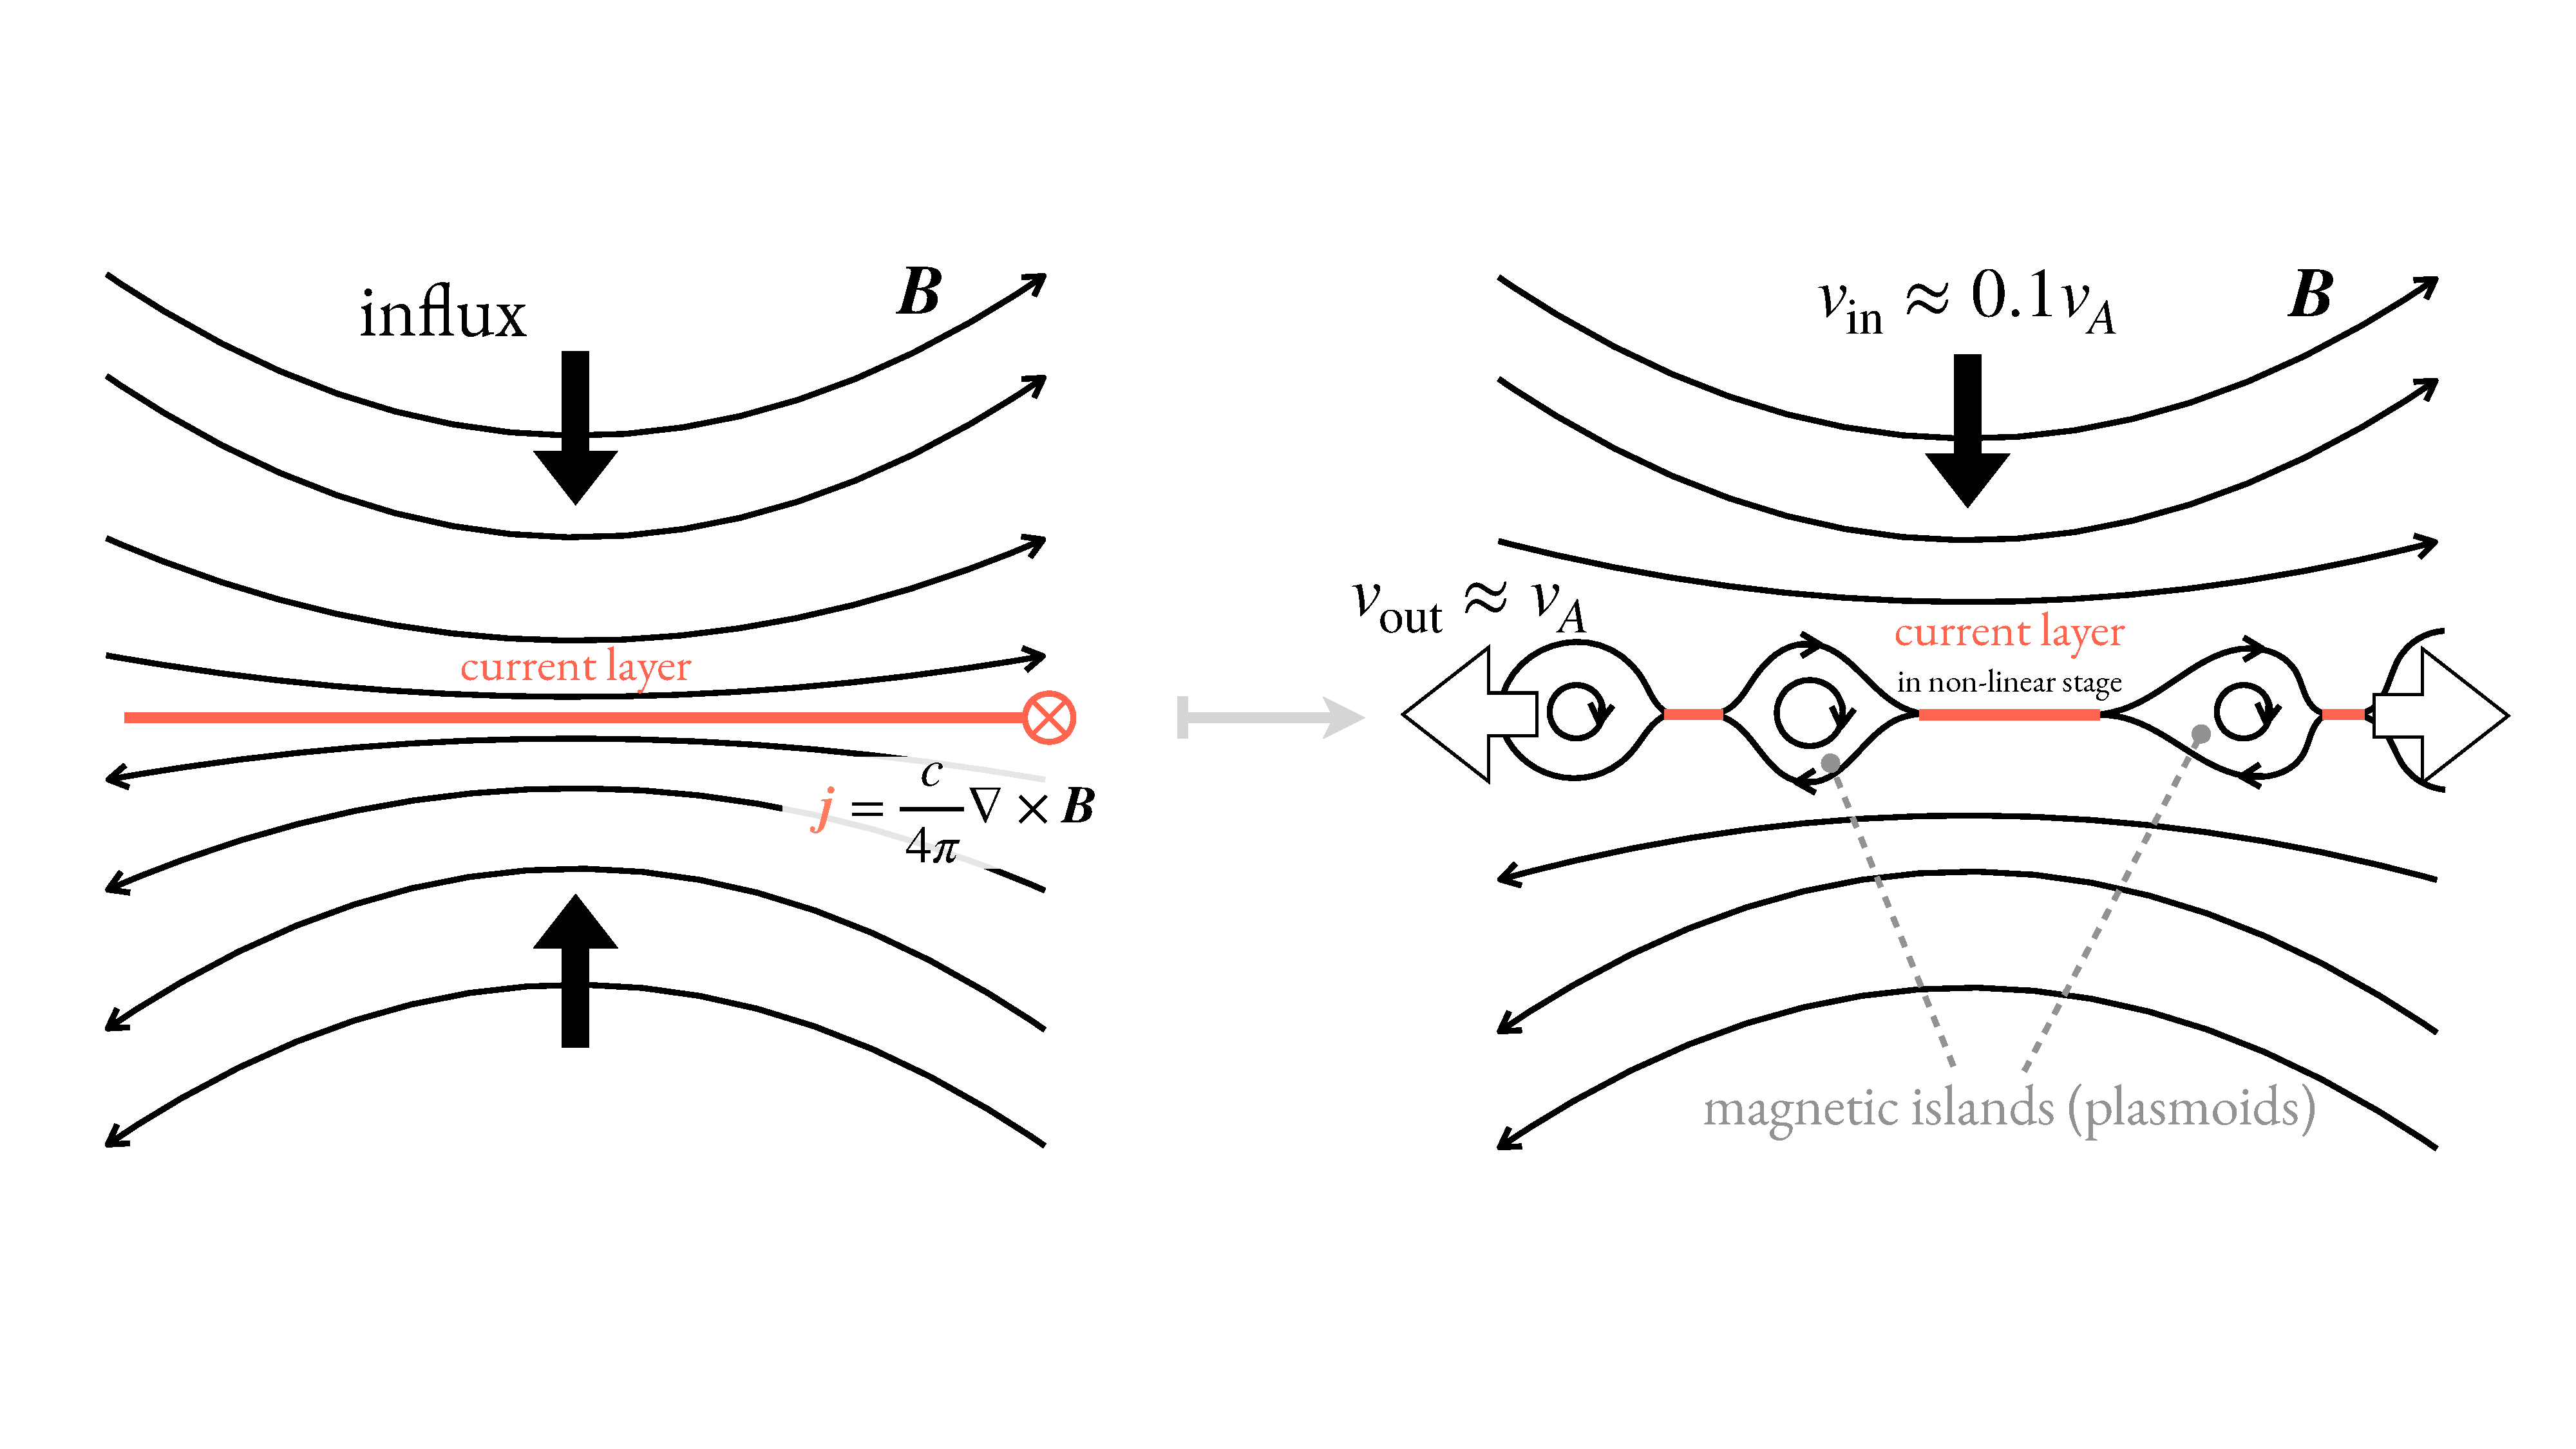
\includegraphics[width=\textwidth,trim={20 150 20 100},clip]{figures/intro/scheme_reconnection.pdf}
    \caption{Schematic illustration of the magnetic reconnection during the onset (left) and the non-linear stage (right). As the current layer disrupts due to tearing instability, reconnection proceeds in the non-linear stage. In this state the dissipation sites in the layer are fragmented, and magnetic islands (plasmoids) are formed moving at near-Alfv\'en velocities and carrying the reconnected magnetic flux and energized plasma. Velocity of the inflow which sets the rate of magnetic energy dissipation is almost ubiquitous, and for collisionless plasma is $v_{\rm in}\approx 0.1v_{A}$.}
    \label{fig:intro-rec}
\end{figure}

During it magnetic energy is dissipated and transformed into plasma kinetic energy; the induced electric field in regions of vanishing magnetic field (inside the red current layer in Figure~\ref{fig:intro-rec}) accelerates charged particles which then shine high-energy photons. What is more critical, is that this process is very rapid. In this non-linear stage the opposing magnetic field lines frozen into plasma inflow at velocities of $0.1 v_A$, with $v_A$ being the Alfv\'en velocity (this was demonstrated in self-consistent kinetic simulations; see, e.g., \citealt{2008ApJ...684.1477Z,2012ApJ...750..129B,2014A&A...570A.111M}). This means, for instance, that a magnetic flux rope may completely dissipate its energy within a few Alfv\'en crossing times of the system. 

In compact objects Alfv\'en velocities approach the speed of light, plasma is often ultra-relativistic, and $\beta$ is no longer a good measure for the level magnetization. Instead, in relativistic plasma astrophysics we often use the \emph{magnetization parameter},
\begin{equation*}
\sigma = \frac{B^2/4\pi}{h},
\end{equation*}
which measures the ratio between the magnetic and plasma enthalpies. In case of relativistically cold plasma $h$ reduces to $\rho c^2$, and $\sigma$ is sometimes referred to as the ``cold’’ magnetization: $\sigma = B^2 / 4\pi \rho c^2$ (where $\rho$ is the matter density). Plasma in the magnetospheres and coronae of compact objects typically have $\sigma\gg1$. This essentially means that the available magnetic energy per each plasma particle far exceeds the particle rest-mass energy. In this regime, the reconnection process is ultra-relativistic, and particles are being accelerated to energies $\gg m c^2$. Studies of magnetic reconnection in $e^\pm$ plasmas in this high-$\sigma$ regime have shown that particles are typically accelerated up to the energies of $\sim \sigma m_e c^2$, forming a hard non-thermal power-law distribution $f(E)\propto E^{-1}\text{-}E^{-2}$ \citep[e.g.,][]{2014PhRvL.113o5005G, 2014ApJ...783L..21S,  2016ApJ...816L...8W}, while a significant fraction of the magnetic energy is being extracted within just a few light-crossing times of the system. All these aspects -- a violently rapid nature and an efficiency in particle acceleration -- have made relativistic reconnection the most likely candidate to explain the underlying plasma microphysics in a variety of compact sources.

In some of the systems the formation of reconnecting current sheets is inevitable. For example, in neutron star and black hole magnetospheres global current layers are self-consistently formed due to the underlying magnetic topology \citep[see, e.g.,][]{2014ApJ...785L..33P,2019PhRvL.122c5101P,2020ApJ...900..100R}. In other scenarios, such as the coronae of x-ray binaries, magnetospheres of magnetars or kink-unstable jets, current sheets can be formed intermittently as a result of larger-scale instabilities or other violent perturbations \citep[see, e.g.,][]{2008ApJ...682..608U,2017ApJ...850..141B,2020ApJ...900L..21Y,2020ApJ...896L..31D}. However, in a general context where plasma is typically disorganized and turbulent the role of the magnetic reconnection that operates at microscopic plasma-scales still remains unclear \citep{2017PhRvL.118e5103Z,2018PhRvL.121y5101C}. 

% In some of the blazar jets, the high-energy cutoff frequencies are much larger, and radiation spectra are more complex, than what we would expect if radiating particles were powered by reconnection. On the contrary, in young $\gamma$-ray pulsars the observed cutoff energy at a few GeV appears to be insensitive to the magnetic field strength in the outer magnetosphere which varies within 3 orders of magnitude among the population. 


Finally, in the vicinity of many of the compact objects radiative reaction, as well as quantum electrodynamic (QED) processes, such as Compton scattering, pair-production/-annihilation, couples photons with plasma and appears to be a vital part of the overall plasma dynamics \citep[for a review see][]{2011SSRv..160...45U}. There has been a handful of computational studies of magnetic reconnection that include some of these effects: \cite{2018JPlPh..84c7501N, 2019MNRAS.482L..60W, 2019ApJ...877...53H, 2019ApJ...870...49S, 2020arXiv201203043N, 2021arXiv210701297M}. These studies demonstrate the wealthy variety of implications of these effects on microscopic dynamics of the reconnection. Nevertheless, it is still largely unclear how the process of magnetic reconnection operates in these extreme conditions, and what are the observational imprints of these QED effects. 

\subsection*{\small \it Young $\gamma$-ray pulsars}

Neutron star magnetospheres are a particularly vivid example of macroscopic systems where reconnecting current layers are formed self-consistently due to the large-scale magnetic topology. \emph{Pulsars} are magnetized neutron stars with the magnetic moment, $\bm{\mu}$, inclined with respect to their spin axis, $\bm{\Omega}$. Magnetospheres of young pulsars are abundant with $e^\pm$ plasma which is extracted from the surface of the star and multiplied in what is known as the pair-cascade  \citep{1969ApJ...157..869G, 1975ApJ...196...51R}. Illustration of the plasma-filled pulsar magnetosphere is shown in Figure~\ref{fig:intro-psr}. The magnetospheric plasma corotates with the field lines, which are ``rigidly attached'' to the perfectly conducting surface of the star, while the induced currents modify the overall structure of magnetic fields.

\begin{figure}[htb]
    \centering
    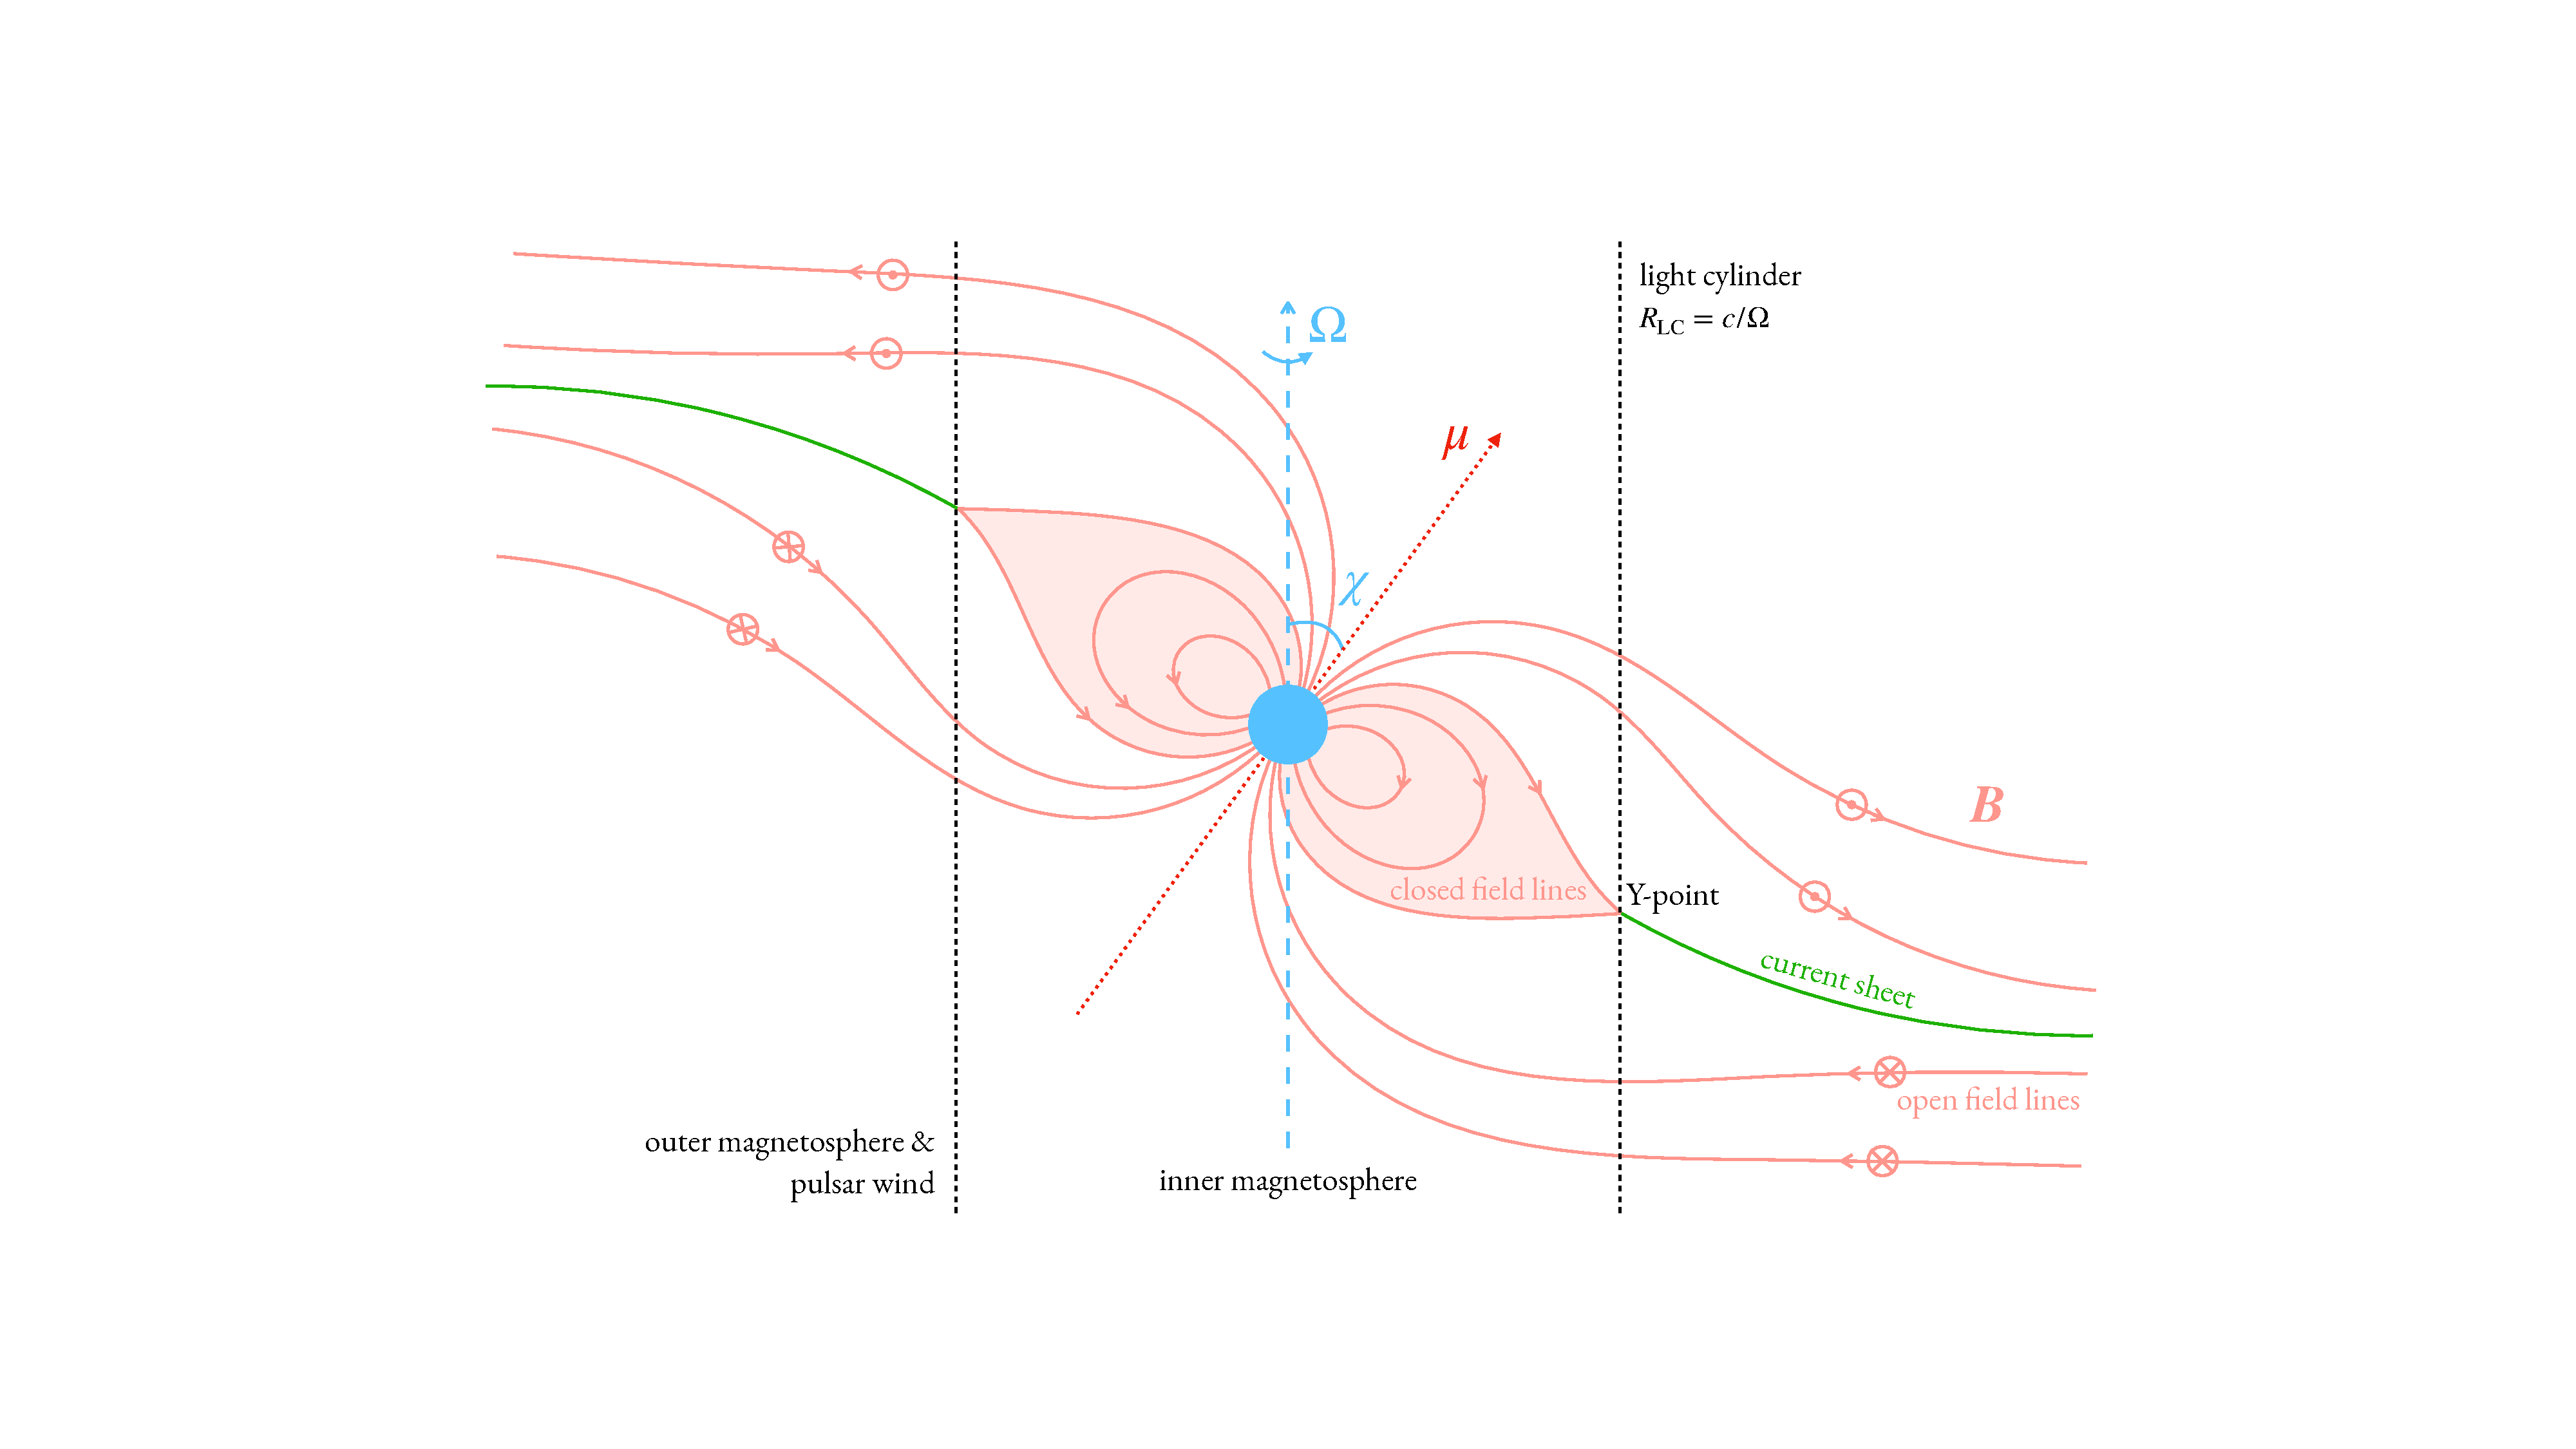
\includegraphics[width=0.8\textwidth,trim={350 150 350 150},clip]{figures/intro/pulsar_side.pdf}
    \caption{Schematic illustration of the structure of neutron star magnetosphere.}
    \label{fig:intro-psr}
\end{figure}

Ultimately, the magnetosphere is separated into two regions (inner and outer) divided by an imaginary surface called \emph{the light cylinder}. This surface corresponds to the distance from the spin axis where plasma can no longer exactly corotate, as that would required faster-than-light velocities: $R_{\rm LC} = c/\Omega$. Magnetic field lines are, thus, subdivided into two groups: the poloidal field lines in the so-called closed zone, and the open field lines in the wind zone. In the wind zone plasma corotates with the almost rigidly rotating magnetic field lines, while at the same time ``slipping'' along them in the outwards direction, forming what is known as the \emph{pulsar wind}. The neutron star loses its rotational energy, carried away via electromagnetic Poynting flux $S_{\hat{r}} = (c/4\pi) E_{\hat{\theta}}B_{\hat{\phi}}$, which, integrated over a sphere which encases the whole magnetosphere is known as the \emph{spin-down power}:\footnote{In reality this value also marginally depends on the inclination angle $\chi$.}

\begin{equation}
    \dot{E} = \frac{\mu^2 \Omega^4}{c^3}.
\end{equation}

\noindent This spin-down power estimates the overall energy budget stored in the form of a magnetic field in the magnetosphere. We can directly estimate the spin-down power by measuring the rate of decay of the spin period of the neutron star, $\dot{P}$, and knowing its moment of inertia, $I$. Then the total spin-down power is empirically equal to $\dot{E} = 4\pi^2 I \dot{P}/P^3$. This makes pulsar magnetospheres uniquely valuable, as we can directly and very precisely measure the energy budget in magnetic field.

In the wind zone open magnetic field lines originating from northern and southern polar caps of the star are separated by a sharp discontinuity: the equatorial current layer (shown with green in Figure~\ref{fig:intro-psr}). Dynamics of this sheet is of particular importance, as it is thought to be the source of the pulsed $\gamma$-ray emission observed in young pulsars \citep{1996A&A...311..172L,2010ApJ...715.1282B,2010MNRAS.404..767C,2011ASSP...21..165A,2012MNRAS.424.2023P,2015MNRAS.448..606C}. Magnetic reconnection in this equatorial layer can power particle acceleration by tapping significant fraction of the $\dot{E}$, which then radiate pulsed emission in x-$\gamma$-rays.

However, there are certain caveats in this model which I will address in some of the future chapters. In particular, the most probable radiation mechanism through which $\gamma$-rays are generated is the synchrotron emission. Pairs accelerated in reconnection up to energies of $E_{\rm max}\sim \sigma_{\rm LC} m_e c^2$ can radiate synchrotron photons up to energies of $\varepsilon_{\rm cut} \propto E_{\rm max}^2 B_{\rm LC}$ (here $\sigma_{\rm LC}$, $B_{\rm LC}$ is the plasma magnetization and the strength of the magnetic field close to the light cylinder).\footnote{$B_{\rm LC}$ can be estimated rather accurately by knowing the magnetic field strength at the surface of the star and the size of the light cylinder.} While the exact value of $\sigma$ at the light cylinder is unknown, we can estimate the scaling with the strength of the magnetic field in the following way: $\sigma_{\rm LC}\propto B_{\rm LC}^2 / \rho_{\rm LC}\propto B_{\rm LC}$. Here we assumed that the plasma density scales as the corresponding Goldreich-Julian density: $\rho_{\rm LC} \propto B_{\rm LC}$. We, thus, find that $\varepsilon_{\rm cut} \propto B_{\rm LC}^3$. Observations, however, show that the cutoff energies vary only marginally from a few to $10$ GeV for the whole population of young pulsars with variations in $B_{\rm LC}$ from $10^3$ to $10^6$ G. If reconnection is indeed responsible for particle acceleration in these systems, it is unclear why the high-energy cutoff is so insensitive to the strength of the magnetic field. 

Moreover, there is an observed dichotomy in $\gamma$-ray spectra for these young pulsars (as shown in Figure~\ref{fig:intro-psrspectra}): high-$\dot{E}$ pulsars, such as Crab, tend to have radiation peaks shifted closer to hard x-rays, while lower-$\dot{E}$ pulsars, such as Vela, peak at energies of a few GeV. The cause of this dichotomy is unclear; and, in general, it is still an open question what physical parameters of the reconnecting current layer determine the position of the $\gamma$-ray peak and the overall form of the spectrum.

\begin{figure}[htb]
    \centering
    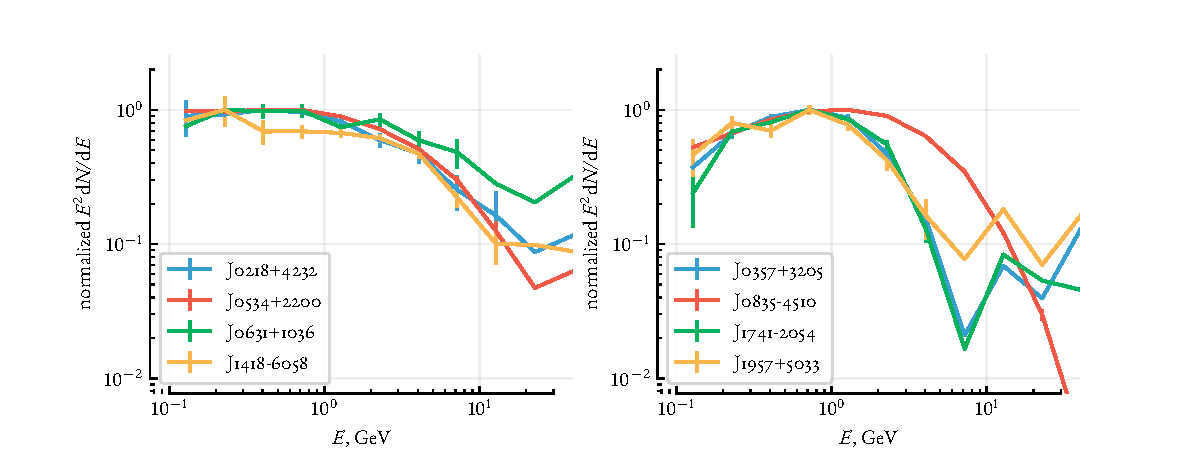
\includegraphics[width=1\textwidth]{figures/intro/highlow_edot.pdf}
    \caption{Schematic illustration of the structure of neutron star magnetosphere.}
    \label{fig:intro-psrspectra}
\end{figure}

\subsection*{\small \it Outline}

Computational high-energy astrophysics attempts to address these and other outstanding questions by self-consistently modeling these systems in numerical simulations. Particle-in-cell (PIC) simulation algorithms, in particular, have proven to be successful in this task both for studying localized microscopic processes (such as isolated reconnection current layers) and also global systems (such as magnetospheres of neutron stars or black holes). In this thesis I present my own contributions in the topic. 

In \S\ref{ch:numerics} I describe the main principles behind numerical techniques used throughout my studies. I present novel algorithms that allow to self-consistently couple some of the mentioned radiative and QED processes to plasma simulations in order to study their effects from first principles. All the other chapters are examples of usage of these methods in studying magnetic reconnection in different regimes in both localized 2D and also global 3D systems.

In \S\ref{ch:plasmoids} I describe the physics behind a new particle acceleration channel in reconnecting current sheets (discovered by \citealt{2018MNRAS.481.5687P}) that was previously overlooked. This channel naturally produces a broken power-law tail, allowing for slow particle acceleration to energies much higher than what was predicted for the relativistic reconnection. I build a theoretical model of this process and compare it against large-scale simulations; this allows to extrapolate the results of localized simulations to real astrophysical systems. This new acceleration channel may help to explain the observed broken power-law spectra in some of the blazar jets. 

\S\ref{ch:pulsar} focuses on global 3D simulations of pulsar magnetospheres. I explore how reconnection occurs in the equatorial current sheet, and what determines the amount of magnetic energy dissipation. I demonstrate that the plasma dynamics of reconnection at microscopically small scales compared to the size of the magnetosphere uniquely determine the total amount of magnetic energy dissipation. I also study the effects of synchrotron cooling on both particle acceleration and high-energy emission, providing a possible hint to explain the observed positions of peaks in $\gamma$-ray pulsars.

Finally, \S\ref{ch:pairproduction} explores the previously unstudied regime of radiative magnetic reconnection with self-consistent pair production. In this process synchrotron photons emitted during particle acceleration and included in the simulations, interact with each other producing electron-positrons pairs. This mechanism feeds the radiated energy back to the sheet in the form of secondary pair-plasma, inhibiting the acceleration efficiency. A process similar to this likely occurs in young pulsars with high spin-down power, and self-consistently controls the plasma density and magnetization in the current layer, explaining the universality of $\gamma$-ray cutoff energies.